\documentclass[a0paper,tikz,border=10pt,landscape]{standalone}
\usepackage[utf8]{inputenc}
\usepackage[sfdefault]{roboto}
\usepackage[T1]{fontenc}

\usepackage{tikz}
\usetikzlibrary{mindmap}
\tikzstyle{every annotation}=[fill=red!20]
\pagestyle{empty}


\begin{document}

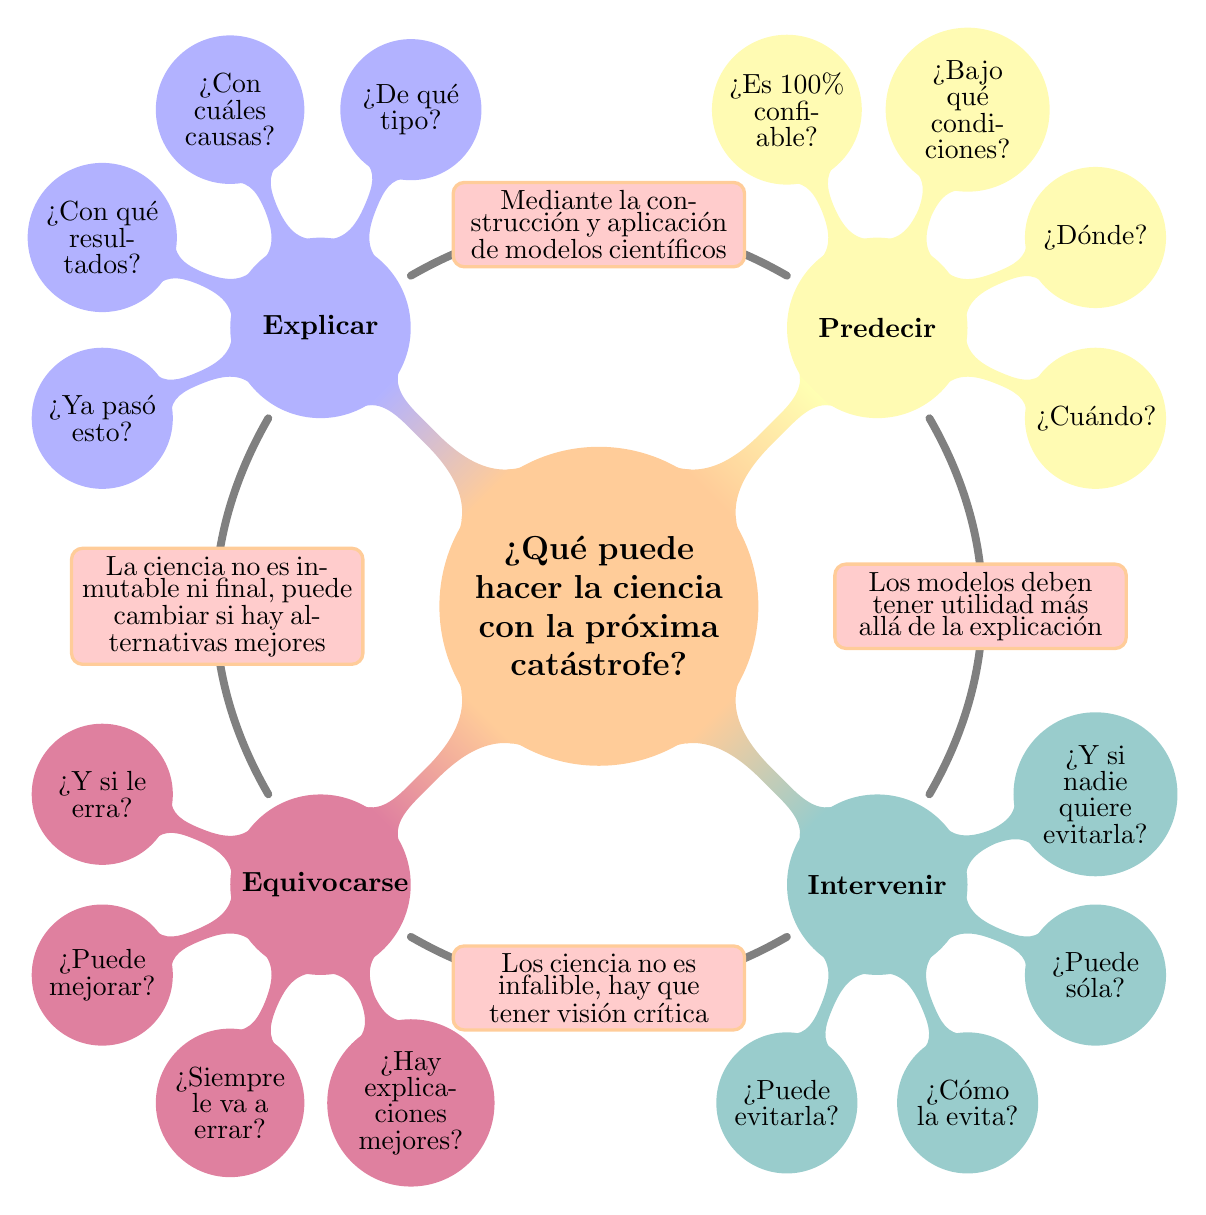
\begin{tikzpicture}[mindmap, grow cyclic, every node/.style=concept, concept color=orange!40, 
    level 1/.append style={level distance=5cm,sibling angle=90},
    level 2/.append style={level distance=3cm,sibling angle=45},]

\node (root) {\textbf{¿Qué puede hacer la ciencia con la próxima catástrofe?}}
    child [concept color=purple!50] { node (m4) {\normalsize{\textbf{Equivocarse}}}
        child { node {\normalsize{¿Y si le erra?}}}
        child { node {\normalsize{¿Puede mejorar?}}}
        child { node {\normalsize{¿Siempre le va a errar?}}}
        child { node {\normalsize{¿Hay explicaciones mejores?}}}
    }
    child [concept color=teal!40] { node (m3) {\normalsize{\textbf{Intervenir}}}
        child { node {\normalsize{¿Puede evitarla?}}}
        child { node {\normalsize{¿Cómo la evita?}}}
        child { node {\normalsize{¿Puede sóla?}}}
        child { node {\normalsize{¿Y si nadie quiere evitarla?}}}
    }
    child [concept color=yellow!30] { node (m2) {\normalsize{\textbf{Predecir}}}
        child { node {\normalsize{¿Cuándo?}}}
        child { node {\normalsize{¿Dónde?}}}
        child { node {\normalsize{¿Bajo qué condiciones?}}}
        child { node {\normalsize{¿Es 100\% confiable?}}}
    }
   child [concept color=blue!30] { node (m1) {\normalsize{\textbf{Explicar}}}
        child { node {\normalsize{¿De qué tipo?}}}
        child { node {\normalsize{¿Con cuáles causas?}}}
        child { node {\normalsize{¿Con qué resultados?}}}
        child { node {\normalsize{¿Ya pasó esto?}}}
    };
    \path[style=concept connection] (m2) edge[bend right] coordinate[midway] (m12) (m1);
    \path[style=concept connection] (m3) edge[bend right] coordinate[midway] (m23) (m2);
    \path[style=concept connection] (m4) edge[bend right] coordinate[midway] (m34) (m3);
    \path[style=concept connection] (m1) edge[bend right] coordinate[midway] (m41) (m4);
    \node [annotation, align=center] at (m12.south) {\normalsize{Mediante la construcción y aplicación de modelos científicos}};
    \node [annotation, align=center] at (m23.east) {\normalsize{Los modelos deben tener utilidad más allá de la explicación}};
    \node [annotation, align=center] at (m34.north) {\normalsize{Los ciencia no es infalible, hay que tener visión crítica}};
    \node [annotation, align=center] at (m41.west) {\normalsize{La ciencia no es inmutable ni final, puede cambiar si hay alternativas mejores}};
\end{tikzpicture}

\end{document}
